\def\rcnn{
    \subsubsection{Mô hình R-CNN}
    Một trong các mô hình đầu tiên ứng dụng deep learning giải quyết bài toán object detection là Regions with CNN features \cite{girshick2014rich} (gọi tắt là R-CNN).
    Tuy nhiên, ở thời điểm mà mô hình R-CNN ra đời, do các mô hình deep learning chưa thật sự phát triển nên mô hình R-CNN không hoàn toàn sử dụng deep learning mà vẫn dựa trên kết quả của thuật toán xử lý ảnh như Graph-Based Image Segmentation \cite{felzenszwalb2004efficient} và Selective Search \cite{uijlings2013selective}.

    \noindent
    \textbf{\textit{Thuật toán Graph-Based Image Segmentation}} \\

    \noindent
    \textbf{\textit{Thuật toán Selective Search}} \\
    
    \noindent
    \textbf{\textit{Kiến trúc mô hình R-CNN}} \\
    Là một trong số các mô hình two-stage, mô hình R-CNN bao gồm hai thành phần: \\
    - Phần Region proposals module mà mô hình R-CNN sử dụng là thuật toán Selective Search ở trên.
    Nhận đầu vào là ảnh, thuật toán Selective Search trả đầu ra là khoảng 2000 khu vực có khả năng có chứa đối tượng và mô hình R-CNN sử dụng các khu vực này làm đầu vào cho thành phần thứ hai. \\
    - Phần Feature extraction module của mô hình R-CNN là một mô hình phân lớp ảnh, cụ thể theo \cite{girshick2014rich} là AlexNet.
    Mô hình R-CNN sử dụng AlexNet nhằm đánh giá xem khu vực đã được đề xuất bởi Selective Search có chứa đối tượng hay không và nếu có thì khu vực đó chứa đối tượng nào. \\

    \begin{figure}[H]
        \centering
        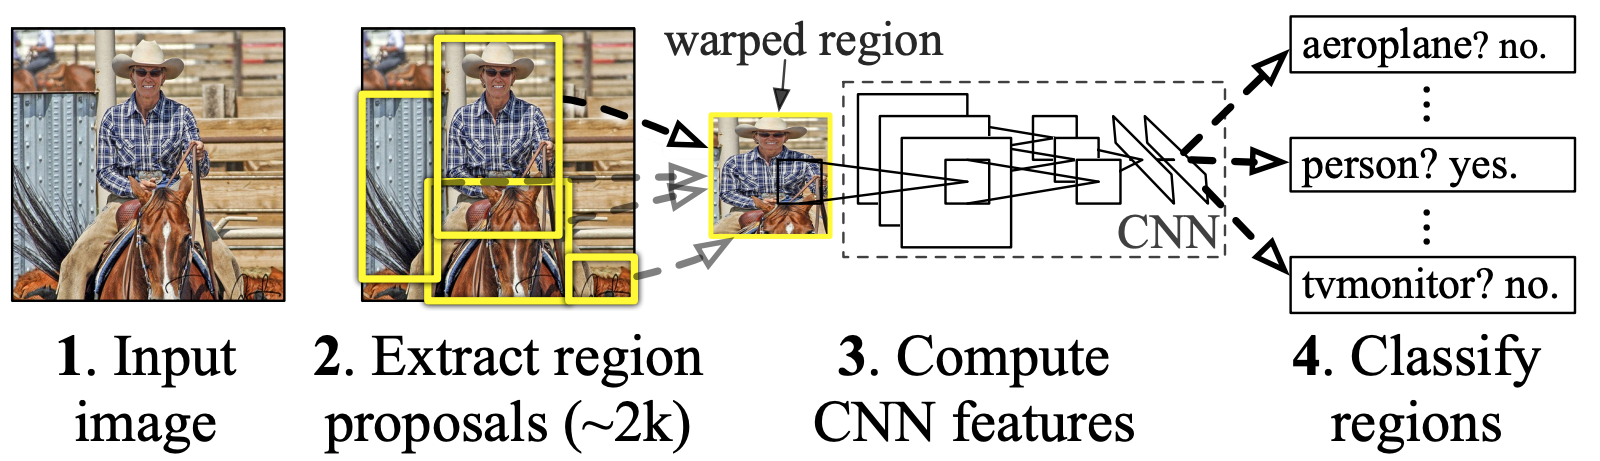
\includegraphics[width=13cm] {images/rcnn_model}
        \caption{Kiến trúc mô hình R-CNN (Nguồn: \cite{girshick2014rich})}
        \label{fig:rcnn_model}
    \end{figure}

    \noindent
    Đối với thành phần Feature extraction module, nhóm tác giả thực hiện hai thí nghiệm: \\
    \textit{Thí nghiệm 1: Finetune mô hình phân lớp CNN} \\
    Nhóm tác giả thay thế lớp fully-connected cuối cùng của mô hình AlexNet (gồm 1000 lớp theo bộ dữ liệu ImageNet) bằng một lớp fully-connected mới (gồm 21 lớp: 20 lớp của bộ dữ liệu VOC và 1 lớp ứng với background).
    Và họ finetune lại mô hình này với thuật toán tối ưu là SGC và learning rate rất nhỏ.
    Các khu vực đã được đề xuất bởi thuật toán Selective Search được sử dụng làm dữ liệu cho bước này, trong đó:
    Những khu vực có chỉ số IoU với groundtruth bounding box >= 0.5 được gán nhãn là lớp của bounding box đó.
    Và ngược lại, sẽ được gán nhãn là lớp background. \\
    TODO Appendix B \\
    Lý do ta cần finetune lại mô hình AlexNet được nhóm tác giả giải thích rằng có những điểm khác nhau giữa bộ dữ liệu pretrained ImageNet và bộ dữ liệu gồm các khu vực được đề xuất bởi Selective Search.

    \noindent
    \textit{Thí nghiệm 2: Xây dựng bộ phân lớp đối tượng bằng SVM} \\
    Với mô hình AlexNet đã được finetune lại như trên, nhóm tác giả sử dụng nó để lấy ra các đặc trưng của ảnh đầu vào và từ đó train các mô hình SVM.
    Mỗi mô hình SVM tương ứng với một lớp đối tượng và mỗi mô hình SVM trả lời cho câu hỏi, đặc trưng của khu vực đó có phải là đối tượng đó hay không.
    Những đặc trưng của khu vực có chỉ số IoU với groundtruth bounding box >= 0.3 sẽ được gán nhãn là lớp của bounding box đó.
    Và ngược lại, những đặc trưng của khu vực có chỉ số IoU với groundtruth bounding box < 0.3 sẽ được gán nhãn không phải là lớp của bounding box đó. \\
    TODO Appendix B \\

    \textit{Bước 3 (Tuỳ chọn)}: Bổ sung thêm hàm loss cải thiện khả năng định vị khu vực \\
    TODO Appendix C \\

    \noindent
    \textbf{\textit{Kết quả của mô hình R-CNN}} \\
    Kết quả của mô hình R-CNN trên bộ dữ liệu VOC 2010 test rất đáng chú ý.
    Trong hình \ref{fig:rcnn_results_3}, ta xét đến hai cấu hình của mô hình R-CNN: \\
    - Cấu hình cơ bản không bao gồm bước Bổ sung thêm hàm loss cải thiện khả năng định vị khu vực được gọi là R-CNN. \\
    - Cấu hình nâng cao Bổ sung thêm hàm loss cải thiện khả năng định vị khu vực được gọi là R-CNN BB. \\
    Với cấu hình cơ bản, R-CNN đạt được chỉ số average precision cao hơn trên tất cả các lớp đối tượng và chỉ số mAP cao hơn 10\% so với các mô hình hiện đại nhất tại thời điểm đó.
    Hơn nữa, với cấu hình R-CNN BB, mô hình còn đạt được chỉ số AP trên tất cả các lớp đối tượng và chỉ số mAP cao hơn 3\% so với cấu hình cơ bản R-CNN.
    \begin{figure}[H]
        \centering
        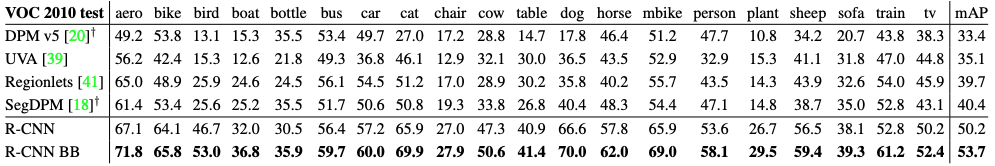
\includegraphics[width=15cm] {images/rcnn_results_3}
        \caption{Kết quả của mô hình R-CNN trên bộ dữ liệu VOC 2010 test. So sánh kết quả của R-CNN và của các mô hình khác nhau (Nguồn: \cite{girshick2014rich})}
        \label{fig:rcnn_results_3}
    \end{figure}
    \noindent
    Ngoài ra, nhóm tác giả cũng nghiên cứu kết quả giữa các cấu hình khác nhau của mô hình R-CNN.
    Trong hình \ref{fig:rcnn_results_1}, nhóm tác giả xét đến hai nhóm cấu hình khác nhau: \\
    - Nhóm cấu hình không finetune và sử dụng đặc trưng ở các vị trí khác nhau cho mô hình phân lớp SVM: \par
    + Cấu hình lấy đặc trưng ở lớp pooling thứ 5: R-CNN ${pool}_{5}$. \par
    + Cấu hình lấy đặc trưng ở lớp fully-connected thứ 6: R-CNN ${fc}_{6}$. \par
    + Cấu hình lấy đặc trưng ở lớp fully-connected thứ 7: R-CNN ${fc}_{7}$. \\
    - Nhóm cấu hình có finetune và sử dụng đặc trưng ở các vị trí khác nhau cho mô hình phân lớp SVM: \par
    + Cấu hình lấy đặc trưng ở lớp pooling thứ 5: R-CNN FT ${pool}_{5}$. \par
    + Cấu hình lấy đặc trưng ở lớp fully-connected thứ 6: R-CNN FT ${fc}_{6}$. \par
    + Cấu hình lấy đặc trưng ở lớp fully-connected thứ 7: R-CNN FT ${fc}_{7}$. \par
    + Cấu hình lấy đặc trưng ở lớp fully-connected thứ 7 kết hợp với hàm loss cải thiện khả năng định vị khu vực: R-CNN FT ${fc}_{7}$ BB. \\
    Với việc finetune lại mô hình với dữ liệu VOC, nhóm cấu hình có finetune mang lại kết quả tốt hơn rất nhiều.
    Trong việc lựa chọn vị trí lấy đặc trưng, vị trí lớp fully-connected thứ 6 là tốt nhất trong nhóm các mô hình không finetune.
    Còn đối với nhóm các mô hình có finetune, vị trí lớp fully-connected thứ 7 là mô hình có kết quả tốt nhất.
    Kết hợp tất cả các kết quả trên, cấu hình R-CNN FT ${fc}_{7}$ BB cho kết quả tốt nhất so sánh với tất cả các cấu hình khác.
    \begin{figure}[H]
        \centering
        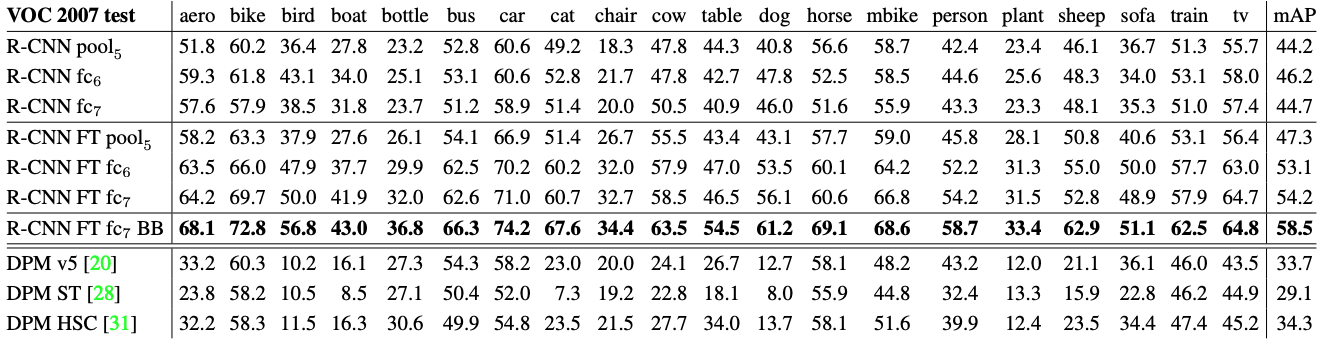
\includegraphics[width=15cm] {images/rcnn_results_1}
        \caption{Kết quả của mô hình R-CNN trên bộ dữ liệu VOC 2007 test. So sánh kết quả của các cấu hình khác nhau của mô hình R-CNN và của mô hình DPM (Nguồn: \cite{girshick2014rich})}
        \label{fig:rcnn_results_1}
    \end{figure}
    \noindent
    Cuối cùng, nhóm tác giả so sánh vai trò của Feature extraction module đối với kết quả chung của mô hình R-CNN.
    Trong hình \ref{fig:rcnn_results_2}, nhóm tác giả xét đến hai mô hình có thể sử dụng trong Feature extraction module: \\
    - Cấu hình sử dụng mô hình AlexNet: R-CNN T-Net và R-CNN T-Net BB. \\
    - Cấu hình sử dụng mô hình VGG16: R-CNN O-Net và R-CNN O-Net BB. \\
    Trong thí nghiệm này, mô hình VGG16 cho kết quả tốt hơn khá nhiều so với mô hình AlexNet.
    \begin{figure}[H]
        \centering
        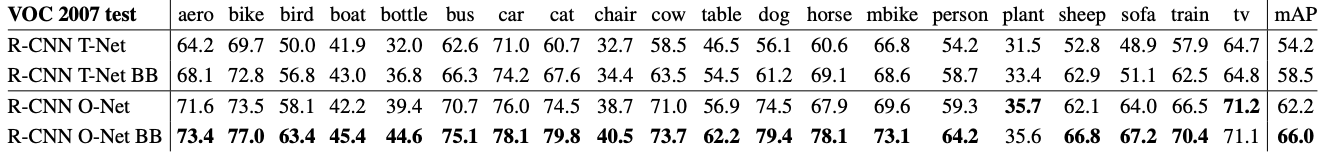
\includegraphics[width=15cm] {images/rcnn_results_2}
        \caption{Kết quả của mô hình R-CNN trên bộ dữ liệu VOC 2007 test (Nguồn: \cite{girshick2014rich})}
        \label{fig:rcnn_results_2}
    \end{figure}

    \noindent
    \textbf{\textit{Vấn đề tồn đọng của mô hình R-CNN}} \\
    Vấn đề lớn nhất của mô hình R-CNN là thời gian mà mô hình cần cho quá trình train và quá trình test là rất lớn.
    Trong quá trình test, mô hình R-CNN sử dụng tới 47 giây để hoàn thành việc xử lý một ảnh.
    Kết quả này khiến cho mô hình R-CNN gần như không có giá trị thực tiễn.
}